\begin{surferPage}[Cubique de Cayley]{La Cubique de Cayley}
   Cette surface cubique (surface de degré $3$) se trouve aussi dans la
    galerie des surfaces simples. 
    En tout, elle a quatre singularités en cône double.
    Elle est nommée d'après Arthur Cayley qui fit de nombreuses recherches sur les cubiques
    au $19$è siècle.
    
     Ce fut cependant Ludwig Schläfli qui, en 1863, classifia en premier ces surfaces de
    manière systématique en fonction de leurs singularités potentielles.
    Ainsi, on peut lire dans son article pourquoi il ne peut y avoir plus de $4$
    points singuliers sur une surface cubique.
    Ce qui donne : $\mu(3)=4$. 
    
    Vers 1900, Felix Klein étudia les formes possibles des surfaces cubiques réelles; 
    son idée fut d'attaquer le problème à partir de la Cubique de Cayley au
    moyen de petites déformations :
    En éclatant les singularités en cône double, en détachant ou en fusionnant certaines parties,
    il parvint en fait à trouver toutes les formes possibles; en voici quelques-unes : 
    \vspace{0.3cm}
     \begin{center}
      \vspace{-0.2cm}
      \begin{tabular}{@{}c@{\ }c@{\ }c@{\ }c@{}}
        \begin{tabular}{@{}c@{}}
          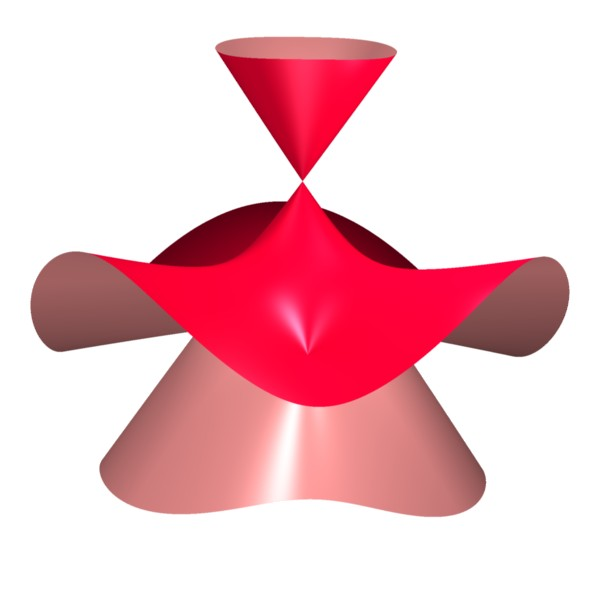
\includegraphics[width=1.35cm]{./../../common/images/cayley_cubic_0}
        \end{tabular}
        &
        \begin{tabular}{@{}c@{}}
          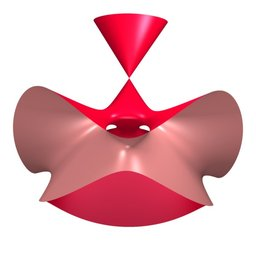
\includegraphics[width=1.35cm]{./../../common/images/cayley_cubic_1}
        \end{tabular}
        &
        \begin{tabular}{@{}c@{}}
          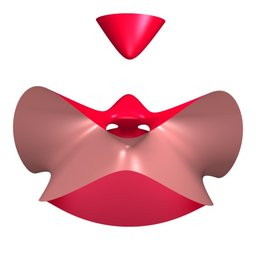
\includegraphics[width=1.35cm]{./../../common/images/cayley_cubic_2}
        \end{tabular}
        &
        \begin{tabular}{@{}c@{}}
          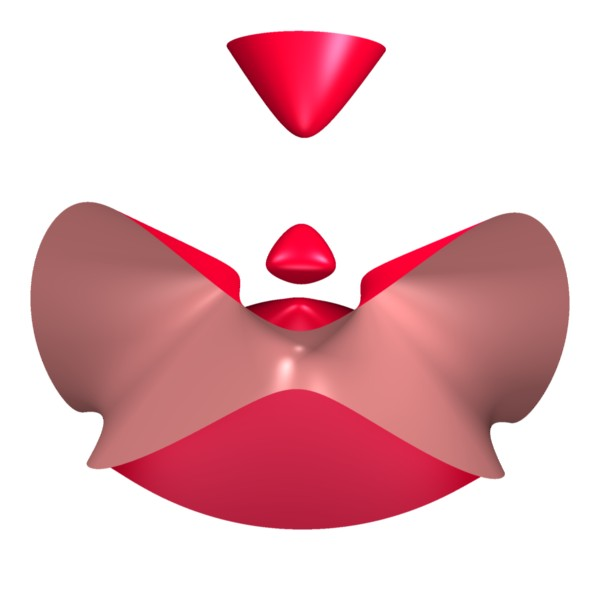
\includegraphics[width=1.35cm]{./../../common/images/cayley_cubic_3}
        \end{tabular}
      \end{tabular}
    \end{center}
\end{surferPage}
